\section{Sabaku no Darude}\label{sabaku-no-darude}

Tags: PC Alias: Il ricercatore della Lore Creatore: Francesco C.
Giocatore: Francesco Curcio Ispirazione: Sabaku no Maiku Luogo: Kos
Razza: Mezz'elfo Classe: Bardo Livello: 10

\section{Sabaku no Darude}\label{sabaku-no-darude-1}

\begin{center}\rule{0.5\linewidth}{0.5pt}\end{center}

\begin{figure}
\centering
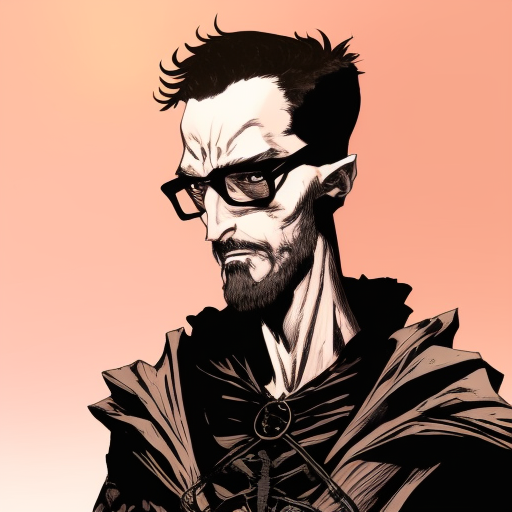
\includegraphics{blkmndy_fantasy_character_with_a_hooded_cape_with_a_beard_with_glasses.png}
\caption{blkmndy\_fantasy\_character\_with\_a\_hooded\_cape\_with\_a\_beard\_with\_glasses.png}
\end{figure}

Informazioni Generali

Età:

Anno di nascita:

Paese di nascita:

Razza: Mezz'elfo

Relazioni:

Alleati:

Nemesi:

Possedimenti importanti:

\begin{center}\rule{0.5\linewidth}{0.5pt}\end{center}

\subsection{1. Descrizione Generale}\label{descrizione-generale}

\begin{center}\rule{0.5\linewidth}{0.5pt}\end{center}

\begin{figure}
\centering
\includegraphics{jflgvgiu98w71.jpg}
\caption{jflgvgiu98w71.jpg}
\end{figure}

Sabaku no Darude è un mezzelfo nato in una landa desertica del
continente. Ha una combinazione di tratti sia umani che elfici, con una
pelle leggermente scura e capelli castani mossi. I suoi occhi, di un
colore ambrato brillante, riflettono la sua passione interiore.

\begin{quote}
``Per chi conosce la Lore. Per chi la sta scoprendo. Per chi la
scoprirà'' - Sabaku no Darude
\end{quote}

\subsection{2. Biografia}\label{biografia}

\begin{center}\rule{0.5\linewidth}{0.5pt}\end{center}

Sabaku no Darude è cresciuto in una landa desertica dopo la morte dei
suoi genitori mercenari quando aveva solo 5 anni. Ha vissuto con il suo
saggio nonno materno, un elfo che gli ha trasmesso l'amore per la musica
e l'arte. Grazie alle storie epiche e alle ballate antiche che ha
ascoltato, Darude ha sviluppato un profondo desiderio di condividerle
con tutte le razze del mondo.

\subsection{3. Carriera}\label{carriera}

\begin{center}\rule{0.5\linewidth}{0.5pt}\end{center}

Per realizzare il suo desiderio di diffondere conoscenza e creare un
legame tra le persone, Darude ha intrapreso un viaggio come bardo
itinerante. Durante i suoi viaggi, esplora nuovi luoghi, impara le
storie locali e interagisce con le diverse culture e razze. Durante
queste esperienze, scrive di sé stesso e degli avvenimenti che gli
accadono intorno, creando un diario di viaggio personale.

Darude si esibisce in vari luoghi, dalle taverne dei villaggi alle corti
dei re, utilizzando la sua abilità musicale e le sue doti di narratore
per coinvolgere il pubblico. La sua musica tocca le corde dell'anima e
le sue storie ispirano gli ascoltatori a guardare al di là delle
differenze e a trovare un terreno comune.

\subsection{4. Personalità}\label{personalituxe0}

\begin{center}\rule{0.5\linewidth}{0.5pt}\end{center}

Darude è una persona gentile e appassionata, con una grande curiosità e
apertura mentale. È rispettoso delle tradizioni locali e cerca sempre di
creare comprensione reciproca tra le diverse razze. La sua passione per
la musica e le storie è contagiosa e porta gioia ovunque vada. Ha
un'anima creativa e un cuore generoso, e cerca di utilizzare le sue
abilità per rendere il mondo un posto migliore.

\subsection{5. Coinvolgimenti in eventi
recenti}\label{coinvolgimenti-in-eventi-recenti}

\begin{center}\rule{0.5\linewidth}{0.5pt}\end{center}

\href{Untitled\%20Database\%2010a4f1e9c7344928a299d9fa00635f6b.csv}{Untitled
Database}

\subsection{6. Scheda personaggio}\label{scheda-personaggio}

\begin{center}\rule{0.5\linewidth}{0.5pt}\end{center}

\href{Info\%20PG\%200f2322afab24429cb360f81d9f366fbc.csv}{Info PG}

\subsubsection{Statistiche e abilità}\label{statistiche-e-abilituxe0}

\begin{center}\rule{0.5\linewidth}{0.5pt}\end{center}

\href{Abilita\%CC\%80\%207e175feb71844b54a1761ee14807b872.csv}{Abilità}

\subsubsection{Lista magie}\label{lista-magie}

\subsection{A. Descrizione originale}\label{a.-descrizione-originale}

\begin{center}\rule{0.5\linewidth}{0.5pt}\end{center}

Sabaku no Darude è un mezzelfo nato in una landa desertica del
continente. I suoi genitori, una madre elfa e un padre umano, erano
mercenari del deserto, ma sono morti quando lui aveva solo 5 anni,
lasciandolo con pochi ricordi di loro. È stato cresciuto dal suo saggio
nonno materno, un elfo che gli ha trasmesso l'amore per la musica e
l'arte. Ha ascoltato le storie epiche e le ballate antiche del
continente, imparando le tradizioni e la saggezza elfica. Le storie
raccontate dal nonno (vissuto oltre 400 anni) hanno suscitato in Darude
il desiderio di condividerle con tutte le razze presenti nel mondo.
Così, ha intrapreso un viaggio come bardo itinerante per esplorare nuovi
luoghi, imparare le loro storie e raccontarle. Durante i suoi viaggi,
Darude si impegna a conoscere diverse culture, interagire con le diverse
razze e preservare le tradizioni locali. Scrive anche di sé stesso e
degli avvenimenti che gli accadono intorno, creando un diario di viaggio
personale. La sua passione è diffondere la conoscenza e creare un legame
tra le persone attraverso la musica e le storie che racconta. Spera di
ispirare gli altri, creare comprensione reciproca e portare gioia
ovunque vada.
